\documentclass[10pt,a4paper]{article}
% Compila con pdflatex (TeX Live), solo paquetes estándar.
\usepackage[utf8]{inputenc}
\usepackage[T1]{fontenc}
\usepackage[spanish,es-noshorthands,es-tabla,es-nodecimaldot]{babel}
\usepackage{lmodern}
\usepackage[margin=1.9cm]{geometry}
\usepackage{amsmath,amssymb,bm}
\usepackage{booktabs,graphicx,caption,enumitem,microtype}
\usepackage[hidelinks]{hyperref}
\setlist{nosep,leftmargin=1.2em}
\captionsetup{font=small,labelfont=bf,skip=3pt}
\setlength{\parskip}{3pt}\setlength{\parindent}{0pt}\emergencystretch=3em
\newcommand{\Xt}{\tilde X}
\newcommand{\R}{\mathbb R}
\newcommand{\E}{\mathbb E}
\DeclareMathOperator{\sign}{sign}
\DeclareMathOperator{\Cov}{Cov}
\graphicspath{{../resultados/}}
% Tiempos medidos con jupyter nbconvert --execute desde un kernel limpio
\newcommand{\tiempoUno}{24\,s}
\newcommand{\tiempoDos}{12\,s}
\newcommand{\tiempoTres}{24\,s}
\newcommand{\equipo}{Linux, Python 3.13}

\title{\vspace{-1.2cm}Taller 1 --- Aprendizaje Automático (2026-2S)\\\large Datos, modelos lineales y decisiones bajo incertidumbre}
\author{Juan José Jiménez Maya}
\date{8 de octubre de 2026}

\begin{document}
\maketitle\vspace{-0.8cm}

\paragraph{Convenciones.} Escribo $\Xt=[\bm 1_N\ X]\in\R^{N\times(D+1)}$ (la matriz $X$ con una columna de unos al inicio), $\theta=(b,w^\top)^\top$ (intercepto y coeficientes en un solo vector) y $P=\operatorname{diag}(0,1,\dots,1)$. Uso los mismos objetivos del notebook de clase~\cite{nbreg}:
\[
F_{\text{lin}}(\theta)=\tfrac{1}{2N}\lVert y-\Xt\theta\rVert_2^2+\tfrac{\lambda_2}{2}\lVert w\rVert_2^2+\lambda_1\lVert w\rVert_1,\qquad
F_{\text{log}}(\theta)=\tfrac1N\textstyle\sum_n\big[\log(1+e^{z_n})-y_nz_n\big]+\tfrac{\lambda_2}{2}\lVert w\rVert_2^2,\quad z_n=\tilde x_n^\top\theta .
\]
El intercepto nunca se penaliza. El código está en el módulo \texttt{mlcore.py} y en tres notebooks ejecutados; las tablas y figuras que cito están en \texttt{resultados/}.

\textbf{Alcance.} Esta entrega incluye el Problema 1 de la parte teórica y los Problemas 4 a 7 de la parte práctica; los Problemas 2 y 3 no están resueltos. Trabajo solo con lo visto en clase: mínimos cuadrados, Ridge, Lasso con umbral suave, regresión logística por descenso por gradiente, validación cruzada y el protocolo de evaluación del taller de vuelos.

% =====================================================================
\section*{Parte I. Fundamentación teórica}

\subsection*{Problema 1. Mínimos cuadrados, Ridge y estabilidad}
El problema pregunta cómo puede ser que un estimador con más sesgo termine estimando mejor. La idea, que justifico en (c), es que Ridge acepta un poco de sesgo a cambio de quitar mucha varianza en las direcciones donde los datos traen poca información, y cuando lo segundo pesa más que lo primero el error total baja.

\textbf{(a) Verosimilitud, gradiente y ecuaciones normales.}
Parto del modelo de las diapositivas 14--15 de la clase~5~\cite{clase5}: cada respuesta es la predicción lineal más un ruido normal y las observaciones son independientes (la densidad normal está en~\cite[cap.~2]{pml1}),
\[ z=Xw+b\,\bm 1_N,\qquad Y_n\mid x_n\sim\mathcal N(z_n,\sigma^2). \]
Al agregar la columna de unos, el intercepto se multiplica por ella y queda dentro de la matriz, de modo que puedo trabajar con un solo vector:
\[ \Xt\theta=\begin{bmatrix}\bm 1_N & X\end{bmatrix}\begin{bmatrix}b\\ w\end{bmatrix}=\bm 1_Nb+Xw=z. \]
La densidad de una observación es la normal evaluada en $y_n$,
\[ p(y_n)=\frac{1}{\sqrt{2\pi\sigma^2}}\exp\!\Big(-\frac{(y_n-z_n)^2}{2\sigma^2}\Big), \]
y como las observaciones son independientes las densidades se multiplican; con el logaritmo el producto se vuelve suma:
\[ \ell(\theta)=\sum_{n=1}^N\Big[-\tfrac12\log(2\pi\sigma^2)-\frac{(y_n-z_n)^2}{2\sigma^2}\Big]=-\frac N2\log(2\pi\sigma^2)-\frac{1}{2\sigma^2}\lVert y-\Xt\theta\rVert_2^2 . \]
Defino $J(\theta)=\frac1{2N}\lVert y-\Xt\theta\rVert_2^2$ y multiplico $\ell$ por $-\sigma^2/N$:
\[ -\frac{\sigma^2}{N}\,\ell(\theta)=\underbrace{\tfrac{\sigma^2}{2}\log(2\pi\sigma^2)}_{\text{no depende de }\theta}+J(\theta). \]
El factor negativo convierte el máximo en mínimo y la constante no mueve el óptimo, así que maximizar $\ell$ equivale a minimizar $J$~\cite[secc.~4.2]{pml1}: con ruido normal, los parámetros más probables son los de menor error cuadrático. El término $\frac{\lambda_2}{2}\lVert w\rVert^2$ de Ridge corresponde a la estimación MAP con previa $w\sim\mathcal N(0,\tau^2I)$ y $\lambda_2=\sigma^2/(N\tau^2)$~\cite[secc.~4.5.3]{pml1}.

Para el gradiente expando $J$ con $\lVert v\rVert^2=v^\top v$:
\[ J(\theta)=\tfrac{1}{2N}(y-\Xt\theta)^\top(y-\Xt\theta)=\tfrac{1}{2N}\big[y^\top y-y^\top\Xt\theta-\theta^\top\Xt^\top y+\theta^\top\Xt^\top\Xt\theta\big]. \]
Los dos términos del medio son el mismo número, porque $y^\top\Xt\theta$ es $1\times1$ y coincide con su transpuesta; queda
\[ J(\theta)=\tfrac{1}{2N}\big[y^\top y-2\,\theta^\top\Xt^\top y+\theta^\top\Xt^\top\Xt\theta\big]. \]
Con las identidades de la diapositiva~9 de la clase~5~\cite{clase5}, $\nabla(\theta^\top a)=a$ y $\nabla(\theta^\top A\theta)=2A\theta$ para $A$ simétrica, y usando que $\Xt^\top\Xt$ es simétrica,
\[ \nabla J(\theta)=\tfrac{1}{2N}\big[-2\Xt^\top y+2\Xt^\top\Xt\theta\big]=\tfrac1N\Xt^\top(\Xt\theta-y). \]
Para la penalización, el cero de $P$ deja por fuera al intercepto: $\theta^\top P\theta=w_1^2+\dots+w_D^2=\lVert w\rVert_2^2$, y como $P$ también es simétrica, $\nabla\big(\frac{\lambda_2}{2}\theta^\top P\theta\big)=\lambda_2P\theta$. Sumando y derivando otra vez,
\[ \nabla F(\theta)=\tfrac1N\Xt^\top(\Xt\theta-y)+\lambda_2P\theta,\qquad \nabla^2F(\theta)=\tfrac1N\Xt^\top\Xt+\lambda_2P. \]
En el mínimo el gradiente se anula; multiplicando por $N$ y factorizando $\theta$ salen las ecuaciones normales:
\[ \Xt^\top(\Xt\theta-y)+N\lambda_2P\theta=0\quad\Longrightarrow\quad \boxed{(\Xt^\top\Xt+N\lambda_2P)\,\theta=\Xt^\top y}. \]
Con $\lambda_2=0$ son las de OLS, y con $\Xt=X$ y $P=I$ es la fórmula de Ridge de la diapositiva~17~\cite{clase5}. Ridge es OLS con $N\lambda_2$ sumado en la diagonal, salvo en la posición del intercepto; en (b) muestro que esa suma basta para que la solución sea única. Las dimensiones: $\Xt$ es $N\times(D+1)$; $\theta$ y $\nabla F$ son $(D+1)\times1$; $y$ y $\Xt\theta$ son $N\times1$; $\Xt^\top\Xt$, $P$ y $\nabla^2F$ son $(D+1)\times(D+1)$.

\textbf{(b) Unicidad y residuos.}
Si $\theta_1$ y $\theta_2$ cumplen ambas $\Xt^\top\Xt\theta=\Xt^\top y$, su diferencia $v=\theta_1-\theta_2$ cumple $\Xt^\top\Xt v=0$. Al multiplicar por $v^\top$ aparece una norma al cuadrado,
\[ v^\top\Xt^\top\Xt v=(\Xt v)^\top(\Xt v)=\lVert\Xt v\rVert_2^2=0\quad\Longrightarrow\quad \Xt v=0. \]
Si las columnas de $\Xt$ son independientes (rango $D+1$, lo que exige $N\ge D+1$), esto solo ocurre con $v=0$. Si alguna columna es combinación de otras existe $v\neq0$ con $\Xt v=0$ y $\theta+v$ también es solución. Por tanto OLS tiene solución única exactamente cuando $\Xt$ tiene columnas independientes (diapositiva~11 de~\cite{clase5}).

Con la matriz de Ridge la misma cuenta da
\[ v^\top(\Xt^\top\Xt+N\lambda_2P)v=\lVert\Xt v\rVert_2^2+N\lambda_2\lVert v_w\rVert_2^2=0 . \]
Ambos sumandos son no negativos, luego ambos son cero. El segundo obliga a $v_w=0$; con eso el primero queda $\Xt v=\bm 1_Nv_b=0$, y $v_b=0$ porque $N\ge1$. Así, con $\lambda_2>0$ Ridge tiene solución única aunque $X$ tenga columnas dependientes y aunque $b$ no esté penalizado.

Sobre los residuos $r=y-\Xt\hat\theta$: en OLS las ecuaciones normales dan $\Xt^\top r=0$, y en Ridge $\Xt^\top r=N\lambda_2P\hat\theta$. La fila de unos sigue dando $\sum_nr_n=0$ porque $P$ tiene un cero en esa posición, pero el resto da $X^\top r=N\lambda_2\hat w\neq0$. Una proyección ortogonal exige que el residuo sea perpendicular a todas las columnas, cosa que OLS cumple (diapositivas 12--13 de~\cite{clase5}) y Ridge no: el ajuste de Ridge es un ajuste encogido y la matriz $H_\lambda=\Xt(\Xt^\top\Xt+N\lambda_2P)^{-1}\Xt^\top$ no es idempotente. Ridge deja deliberadamente parte de la señal sin explicar a cambio de coeficientes más pequeños.

\textbf{(c) Sesgo y varianza.} Aquí ``sesgo'' significa el error promedio del estimador, no el intercepto $b$, y uso la descomposición $\text{ECM}=\text{varianza}+\text{sesgo}^2$ de~\cite[secc.~4.7.6]{pml1}. Supongo $b=0$, $X$ fija y de rango completo, e $y=Xw^\star+\varepsilon$ con $\E[\varepsilon]=0$ y $\Cov(\varepsilon)=\sigma^2I_N$.

Sin intercepto, $P$ es la identidad y $\hat w=AX^\top y$ con $A=(X^\top X+N\lambda_2I)^{-1}$, que es simétrica. Como las matrices son fijas y $\E[y]=Xw^\star$, se tiene $\E[\hat w]=AX^\top Xw^\star$. Despejando $X^\top X=A^{-1}-N\lambda_2I$ obtengo $AX^\top X=I-N\lambda_2A$, de donde
\[ \text{sesgo}=\E[\hat w]-w^\star=(I-N\lambda_2A)w^\star-w^\star=-N\lambda_2Aw^\star . \]
Para la covarianza uso $\Cov(My)=M\Cov(y)M^\top$ con $M=AX^\top$: $\Cov(\hat w)=AX^\top(\sigma^2I)XA=\sigma^2AX^\top XA$.

Todo se separa por direcciones propias. Escribo $X^\top X=\sum_kd_kv_kv_k^\top$, donde $d_k>0$ mide cuánta información hay en la dirección $v_k$; con $\kappa=N\lambda_2$ y $\alpha_k=v_k^\top w^\star$, $A=\sum_k\frac{1}{d_k+\kappa}v_kv_k^\top$ y
\[ \text{sesgo}_k=-\frac{\kappa}{d_k+\kappa}\,\alpha_k,\qquad \operatorname{Var}_k=\sigma^2\frac{d_k}{(d_k+\kappa)^2}. \]
Es decir, en cada dirección Ridge multiplica la estimación de OLS por $d_k/(d_k+\kappa)\in(0,1)$: casi no toca las direcciones con mucha información y encoge fuerte las de $d_k$ pequeño, que son las de variables casi colineales. En los extremos, con $\lambda_2\to0$ el sesgo desaparece y $\operatorname{Var}_k\to\sigma^2/d_k$, que es la varianza de OLS y se dispara cuando $d_k$ es pequeño; con $\lambda_2\to\infty$, $\hat w\to0$, el sesgo tiende a $-\alpha_k$ y la varianza a cero.

Para ver cuándo gana Ridge comparo el error de la dirección $k$ (sesgo$^2$ más varianza) con el de OLS:
\[ \frac{\kappa^2\alpha_k^2+\sigma^2d_k}{(d_k+\kappa)^2}<\frac{\sigma^2}{d_k}. \]
Multiplicando en cruz, cancelando $\sigma^2d_k^2$ y dividiendo por $\kappa>0$ queda
\[ \kappa\,(d_k\alpha_k^2-\sigma^2)<2\sigma^2d_k . \]
Para $\kappa$ pequeño la desigualdad se cumple siempre, así que existe algún $\lambda_2$ que mejora a OLS. En cambio, si la dirección tiene señal fuerte ($d_k\alpha_k^2>\sigma^2$) y $\kappa$ es grande, la desigualdad falla: bajar la varianza no garantiza bajar el error con cualquier regularización, porque el sesgo$^2$ sigue creciendo. En cuanto a estabilidad, $\operatorname{Var}_k\le\sigma^2/(4N\lambda_2)$, de modo que Ridge acota la inestabilidad de las direcciones casi colineales. La simulación del Problema 5 pone esto a prueba.

% =====================================================================
\section*{Parte II. Implementación y experimentación}

\subsection*{Problema 4. Modelos desde cero y verificación numérica}
\textbf{(a) Implementación.}
Todos los modelos viven en \texttt{mlcore.py}, escrito con NumPy, sin inversas explícitas, sin diferenciación automática y sin optimizadores genéricos. Cada clase separa el entrenamiento (\texttt{fit}), la predicción (\texttt{predict}, \texttt{predict\_proba}) y la evaluación (\texttt{objective}, \texttt{log\_loss}).

OLS usa \texttt{np.linalg.lstsq}, que con columnas repetidas devuelve la solución de norma mínima; guardo además el rango. Ridge resuelve con \texttt{np.linalg.solve} el sistema $(\Xt^\top\Xt+N\lambda_2P)\theta=\Xt^\top y$ del Problema 1(a), siguiendo el Algoritmo~1 de la clase~5: se resuelve el sistema, no se invierte la matriz~\cite{clase5}.

Para la regresión lineal y la logística (con L2 opcional) uso descenso por gradiente, $\theta\leftarrow\theta-\eta\nabla F(\theta)$, como \texttt{LinearRegressionScratch} y \texttt{LogisticRegressionScratch} del notebook de clase~\cite{nbreg} y el Algoritmo~2 de~\cite{clase5}. La tasa no la fijo a mano: tomo $\eta=1/L$ con $L$ el mayor autovalor del Hessiano, que es $\sigma_{\max}(\Xt)^2/N+\lambda_2$ en el caso lineal y $\sigma_{\max}(\Xt)^2/(4N)+\lambda_2$ en el logístico (en el Hessiano $\frac1N\Xt^\top S\Xt$ de la diapositiva~29, $p_n(1-p_n)\le1/4$). Con ese paso el objetivo baja en cada iteración.

Lasso sigue la actualización de \texttt{fit\_regularized} de clase~\cite{nbreg}. Como $\lambda_1\lVert w\rVert_1$ no es derivable en cero, cada iteración da un paso de gradiente sobre la parte suave, $u=\theta-\eta\nabla f(\theta)$, y luego aplica a cada $w_j$ el umbral suave $S(u_j,\eta\lambda_1)=\sign(u_j)\max(|u_j|-\eta\lambda_1,0)$, sin tocar $b$. Cuando $|u_j|\le\eta\lambda_1$ el coeficiente queda en cero exacto, de modo que los ceros los produce el algoritmo y no un redondeo posterior.

El criterio de parada es el de \texttt{fit\_regularized}: $\lVert\theta^+-\theta\rVert_2/\eta<\texttt{tol}$. Sin L1 coincide con la norma del gradiente; en Lasso es el residuo de la actualización proximal, incluido $b$. Uso tolerancia $10^{-8}$ y un máximo de $5\cdot10^4$ a $2\cdot10^5$ iteraciones. En cada iteración guardo el objetivo completo, y al final el número de iteraciones y el motivo de parada; también reviso dimensiones, valores finitos e hiperparámetros, y cada \texttt{fit} arranca de $\theta=0$.

En la Figura~\ref{fig:p4} las tres corridas paran por tolerancia con el objetivo bajando en cada paso. Para Ridge, la distancia al mínimo exacto calculado con \texttt{solve} llega al nivel del redondeo, lo que valida al mismo tiempo el gradiente y las ecuaciones normales.

\begin{figure}[h]\centering
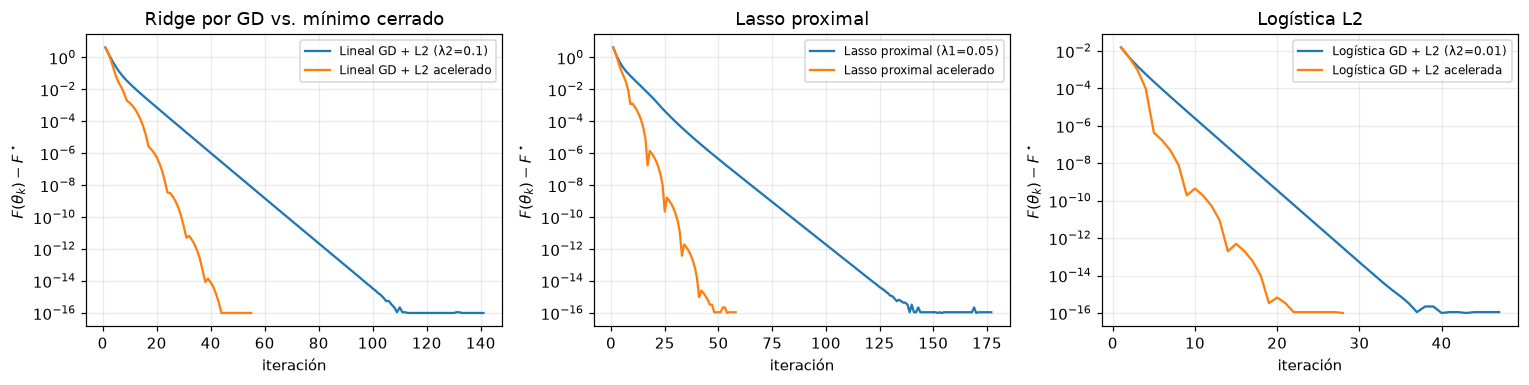
\includegraphics[width=0.95\linewidth]{p4_convergencia.png}
\caption{Historial de convergencia ($\eta=1/L$, parada por tolerancia): Ridge por GD frente a su mínimo exacto, Lasso proximal y logística L2.}\label{fig:p4}
\end{figure}

\textbf{(b) Pruebas automáticas.}
El Notebook~1 contiene 30 pruebas; cada una compara un valor con un umbral fijo y un \texttt{assert} detiene la ejecución si alguna falla. Las 30 pasan, y la tabla completa está en \texttt{p4\_pruebas\_numericas.csv}.

Los gradientes los comparo con diferencias centrales, $g_j\approx[F(\theta+he_j)-F(\theta-he_j)]/(2h)$ con $h=10^{-6}$, en tres puntos $\theta\sim U(-1,1)$ e incluyendo $b$ y L2. El peor error relativo es $\delta_g\le2.5\times10^{-10}$, lejos de la meta de $10^{-5}$; la parte L1 no la verifico numéricamente en cero.

Para la estabilidad numérica evalúo la sigmoide y la pérdida en $z\in\{\pm1000,\pm100,\pm1,0\}$ con ambas etiquetas, usando las fórmulas del notebook de clase~\cite{nbreg}: $\sigma(z)=\exp(-\log(1+e^{-z}))$ y la pérdida $\log(1+e^{-z})$ si $y=1$ o $\log(1+e^{z})$ si $y=0$, ambas con \texttt{np.logaddexp(0,u)}$=\log(e^0+e^u)$, que nunca calcula una exponencial enorme. Todos los valores son finitos y coinciden exactamente con los valores de referencia, sin recortar el score.

También pruebo casos difíciles. Con una columna duplicada, OLS detecta rango $D$, cumple $\lVert\Xt^\top r\rVert=7\times10^{-14}$ y conserva las predicciones, y Ridge tiene residuo de ecuaciones normales $4\times10^{-14}$ y asigna el mismo coeficiente a las dos copias, como anticipa 1(b). En un diseño ortogonal ($X^\top X/N=I$) Lasso reproduce el umbral suave $S(s,\lambda_1)$ con $s=X^\top y/N$ (error $9\times10^{-16}$); en un diseño correlacionado compruebo la optimalidad con el residuo proximal, $\lVert\theta^+-\theta\rVert/\eta=9\times10^{-12}$, es decir, la solución es un punto fijo del algoritmo. Por último, guardar y cargar los parámetros en JSON no altera las predicciones, las probabilidades están en $[0,1]$ y suman 1, y cambiar $\tau$ no modifica \texttt{predict\_proba} ni la log-loss.

\textbf{(c) Comparación con scikit-learn 1.9.1.}
Comparo con scikit-learn~\cite{sklearn} sobre las mismas matrices ya preparadas. Como scikit-learn escribe los objetivos con otra escala, multiplico el mío por la constante adecuada para igualarlos (Tabla~\ref{tab:equiv}); es la tabla de equivalencias del notebook de clase~\cite{nbreg} con la derivación explícita.

\begin{table}[h]\centering\small
\caption{Correspondencia entre mis hiperparámetros y los de scikit-learn 1.9.1 (intercepto nunca penalizado).}\label{tab:equiv}
\begin{tabular}{llll}\toprule
Estimador & Objetivo de scikit-learn & Multiplico el mío por & Equivalencia\\\midrule
\texttt{LinearRegression} & $\lVert y-Xw-b\rVert^2$ & $2N$ & sin penalización\\
\texttt{Ridge} & $\lVert y-Xw-b\rVert^2+\alpha\lVert w\rVert^2$ & $2N$ & $\alpha=N\lambda_2$\\
\texttt{Lasso} & $\frac1{2N}\lVert y-Xw-b\rVert^2+\alpha\lVert w\rVert_1$ & $1$ & $\alpha=\lambda_1$\\
\texttt{LogisticRegression} & $C\sum_n\ell_n+\frac12\lVert w\rVert^2$ & $1/(N\lambda_2)$ & $C=1/(N\lambda_2)$\\\bottomrule
\end{tabular}\end{table}

Por ejemplo, para Ridge mi objetivo es $\frac1{2N}\lVert r\rVert^2+\frac{\lambda_2}{2}\lVert w\rVert^2$; al multiplicarlo por $2N$ queda $\lVert r\rVert^2+N\lambda_2\lVert w\rVert^2$, que es el de scikit-learn con $\alpha=N\lambda_2$. Las demás filas se obtienen igual. Como $\alpha$ de Ridge y $C$ dependen de $N$, repito la comparación con $N$ y con $N/2$ filas, recalculando la equivalencia en cada caso; para la logística sin penalizar uso \texttt{C=np.inf}.

En los 12 contrastes la diferencia relativa de objetivo no pasa de $2.2\times10^{-16}$ y la de predicciones o probabilidades no pasa de $9.7\times10^{-9}$, con meta $10^{-4}$; en la logística comparo probabilidades y no solo etiquetas. El único caso con coeficientes distintos es Lasso con una columna duplicada, que tiene infinitas soluciones porque solo queda determinada la suma de los dos coeficientes: scikit-learn da $(0.58,0.89)$ y mi gradiente proximal $(0.73,0.73)$, con el mismo objetivo y las mismas predicciones (error $3.6\times10^{-12}$). Ahí comparar coeficientes uno a uno daría una falsa alarma, y lo que tiene sentido es comparar el objetivo y las predicciones.

% ---------------------------------------------------------------------
\subsection*{Problema 5. Simulación de sesgo, varianza y selección}
Con un solo conjunto de datos no se puede separar el sesgo de la varianza, así que repito muchas veces el mismo experimento cambiando únicamente el ruido. El promedio de las réplicas muestra cuánto se equivoca el modelo en promedio y su dispersión muestra cuánto cambia de una réplica a otra.

\textbf{(a) Diseño.}
Sigo el enunciado: $N=120$, $D=20$, $M=1000$, $R=40$, $\sigma^2=1$, filas $x_n\sim\mathcal N(0,\Sigma_\rho)$~\cite[secc.~3.2]{pml1} con cuatro bloques de 5 variables y correlación $\rho\in\{0,0.9\}$ dentro de cada bloque, y coeficientes verdaderos $w^\star_1=3$, $w^\star_6=-2$, $w^\star_{11}=1.5$, $w^\star_{16}=-1$ (uno por bloque), sin intercepto ni escalador. De la semilla maestra 2026 derivo subsemillas para $X$, para $X_*$ y para cada uno de los 40 ruidos, y las guardo en \texttt{p5\_subsemillas.json} para poder repetir cualquier réplica por separado. Con $X$ y $X_*$ fijas ajusto OLS, Ridge y Lasso con mis clases para cada $\lambda\in\{10^{-3},\dots,10\}$ y cada una de las 40 respuestas.

\textbf{(b) Descomposición del error.}
En cada punto de auditoría $m$, $f^\star_m$ es el valor verdadero, $\hat f_{rm}$ la predicción de la réplica $r$ y $\bar f_m$ el promedio de las 40. $\hat B^2$ mide la distancia del promedio a la verdad, $\hat V$ la dispersión de las réplicas alrededor de su promedio y $\hat E_f$ el error total.

La identidad $\hat E_f=\hat B^2+\hat V$ es exacta. Al expandir $(\hat f_{rm}-f^\star_m)^2=\big((\hat f_{rm}-\bar f_m)+(\bar f_m-f^\star_m)\big)^2$ aparece el término cruzado $\tfrac2R\sum_r(\hat f_{rm}-\bar f_m)(\bar f_m-f^\star_m)$, que se anula porque $\sum_r(\hat f_{rm}-\bar f_m)=0$; esto requiere el factor $1/R$, con $1/(R-1)$ no cierra. Es la cuenta $\text{ECM}=\text{varianza}+\text{sesgo}^2$ de~\cite[secc.~4.7.6]{pml1} con promedios sobre réplicas, y numéricamente se cumple hasta el redondeo. Si lo que interesa es predecir una respuesta nueva $y_*=f^\star+\varepsilon_*$, el ruido $\varepsilon_*$ es independiente de todo lo anterior e impredecible, y el error esperado pasa a ser $\hat E_f+\sigma^2$. Hay que tener en cuenta además que $\bar f_m$ se calcula con solo 40 réplicas y tiene su propio ruido; por eso OLS, que es insesgado, muestra $\hat B^2\approx0.004$--$0.007$ y no 0.

\begin{table}[h]\centering\small
\caption{Error en $X_*$ (en negrita, el menor $\hat E_f$ de cada modelo y escenario). OLS: $\hat E_f=0.201$ ($\rho=0$) y $0.200$ ($\rho=0.9$), con $\hat V\approx0.195$.}\label{tab:p5}
\begin{tabular}{l ccc ccc | ccc ccc}\toprule
& \multicolumn{6}{c|}{$\rho=0$} & \multicolumn{6}{c}{$\rho=0.9$}\\
& \multicolumn{3}{c}{Ridge} & \multicolumn{3}{c|}{Lasso} & \multicolumn{3}{c}{Ridge} & \multicolumn{3}{c}{Lasso}\\
$\lambda$ & $\hat B^2$ & $\hat V$ & $\hat E_f$ & $\hat B^2$ & $\hat V$ & $\hat E_f$ & $\hat B^2$ & $\hat V$ & $\hat E_f$ & $\hat B^2$ & $\hat V$ & $\hat E_f$\\\midrule
$10^{-3}$ & .007 & .194 & .201 & .007 & .191 & .198 & .003 & .191 & .195 & .004 & .186 & .190\\
$10^{-2}$ & .008 & .189 & \textbf{.197} & .006 & .164 & .170 & .016 & .160 & \textbf{.176} & .005 & .123 & .128\\
$10^{-1}$ & .194 & .150 & .344 & .043 & .053 & \textbf{.096} & .384 & .065 & .449 & .050 & .054 & \textbf{.104}\\
$1$ & 4.36 & .039 & 4.40 & 4.65 & .032 & 4.68 & 1.45 & .021 & 1.48 & 2.76 & .032 & 2.79\\
$10$ & 13.2 & .001 & 13.2 & 16.0 & .000 & 16.0 & 7.26 & .003 & 7.27 & 15.8 & .000 & 15.8\\\bottomrule
\end{tabular}\end{table}

En la Tabla~\ref{tab:p5}, al subir $\lambda$ la varianza siempre baja y el sesgo$^2$ sube. El mejor $\hat E_f$ aparece en valores intermedios ($\lambda_2=0.01$ para Ridge y $\lambda_1=0.1$ para Lasso), ambos por debajo de OLS (0.20), mientras que desde $\lambda=1$ domina el sesgo y los dos quedan muy por encima de OLS.

Contrasté Ridge con las fórmulas de 1(c). La media empírica se aleja de $AX^\top Xw^\star$ lo que cabe esperar con 40 réplicas (del orden de $\sqrt{\operatorname{tr}\Cov/R}$), y la varianza total empírica $\operatorname{tr}\Cov$ sigue a la teórica $\operatorname{tr}(\sigma^2AX^\top XA)$ (por ejemplo, 1.59 frente a 1.50 con $\rho=0.9$ y $\lambda_2=10^{-3}$), bajando con ella al aumentar $\lambda_2$. Con $\rho=0.9$ el número de condición de $X^\top X$ es 145, frente a 4.5 con $\rho=0$. En la dirección de menor autovalor ($d=5.1$) OLS tiene varianza 0.194 y $\lambda_2=0.01$ la reduce a 0.128 con un sesgo de 0.33, mientras que en la dirección más grande ($d=747$) el sesgo es casi nulo. Coincide con lo que predice 1(c): el encogimiento se concentra en las direcciones inestables.

\textbf{(c) Selección con Lasso.}
Antes de mirar resultados fijé la tolerancia $|\hat w_j|>10^{-8}$ para considerar elegida una variable. La precisión es la fracción de elegidas que son relevantes, la sensibilidad es la fracción de las 4 relevantes que fueron elegidas, y un bloque cuenta como recuperado si se elige al menos una de sus cinco variables.

Sin correlación, $\lambda_1=1$ acierta el soporte exacto en el 82.5\% de las réplicas (precisión 1, sensibilidad 0.96), pero con $\hat E_f=4.68$. El mejor valor para predecir, $\lambda_1=0.1$, elige 8.4 variables en promedio (precisión 0.49, sensibilidad 1) y no acierta el soporte exacto en ninguna réplica. Con $\rho=0.9$ y $\lambda_1=1$ la sensibilidad individual cae a 0.76 aunque la de bloque es 1.0, con 0.98 sustituciones por réplica: Lasso toma otra variable del mismo bloque en lugar de la verdadera. Con esa correlación ningún $\lambda$ acierta el soporte exacto, y $\lambda_1=10$ anula todos los coeficientes.

\begin{figure}[h]\centering
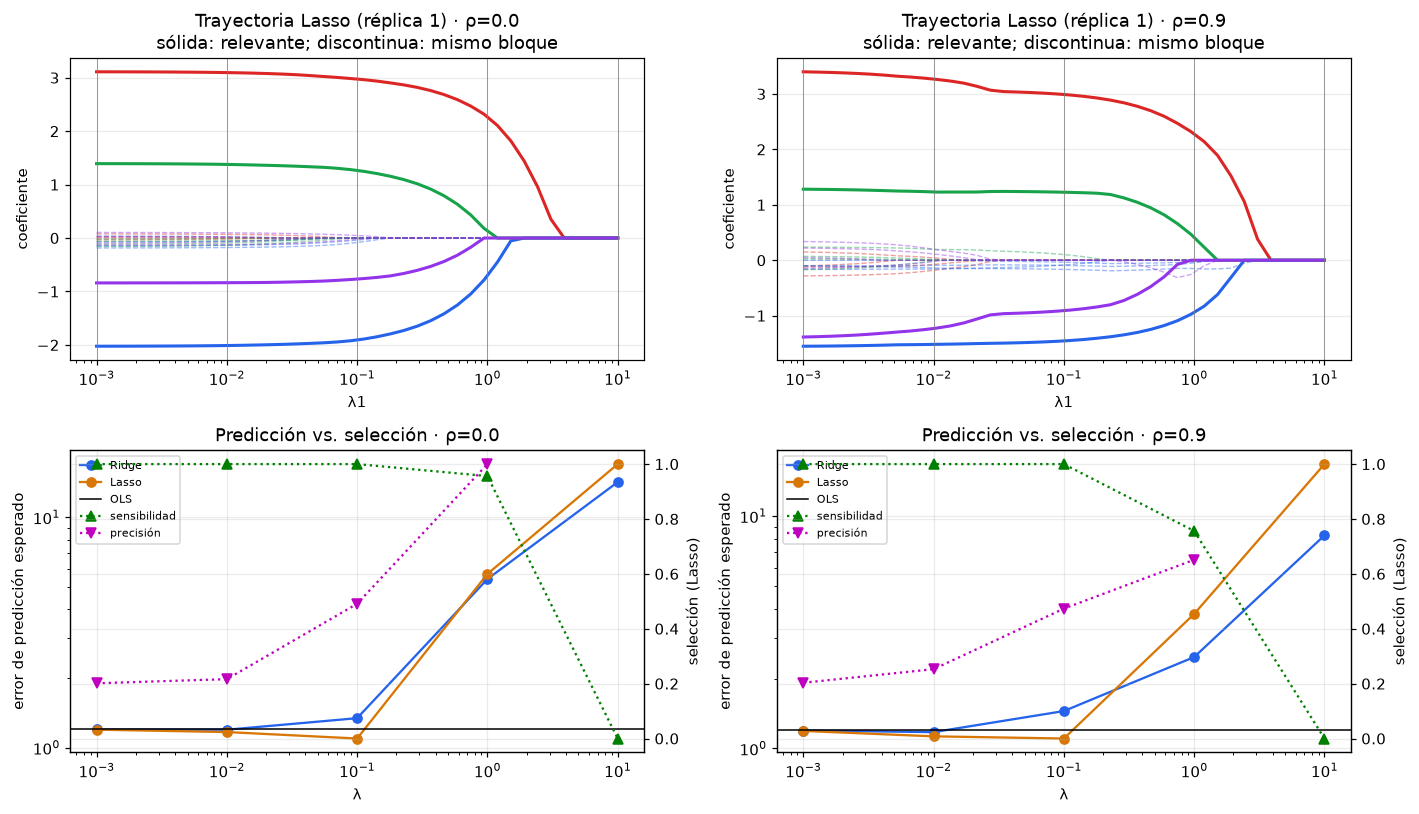
\includegraphics[width=0.93\linewidth]{p5_trayectorias_seleccion.png}
\caption{Arriba: trayectorias de Lasso (réplica 1); línea sólida = variable relevante, discontinua = otra variable de su bloque. Abajo: error de predicción esperado frente a sensibilidad y precisión.}
\end{figure}

\textbf{(d) Respuestas con evidencia.}
La regularización no reduce sesgo y varianza a la vez: en la Tabla~\ref{tab:p5} una baja mientras el otro sube. El único descenso conjunto (Lasso, $\rho=0$, de $10^{-3}$ a $10^{-2}$, con $\hat B^2$ pasando de 0.007 a 0.006) es del tamaño del ruido de promediar 40 réplicas. Lo que hace la regularización es intercambiar varianza por sesgo, y ese intercambio solo mejora el error total en un rango intermedio de $\lambda$.

Predecir mejor tampoco implica recuperar el soporte. El Lasso que mejor predice nunca acierta el soporte exacto, y el que mejor lo acierta tiene un error unas 49 veces mayor; seleccionar variables y predecir son objetivos distintos.

Una variable irrelevante reemplaza a una relevante cuando está muy correlacionada con ella, como en el caso $\rho=0.9$. En la muestra $x_j\approx x_1$, así que $w_jx_j$ aporta casi lo mismo con una penalización parecida; la variable no está en el modelo verdadero pero sí sirve para predecir, y por eso la selección cambia de una réplica a otra.

% ---------------------------------------------------------------------
\subsection*{Problema 6. Regresión reproducible sobre Airfoil}
\textbf{(a) Auditoría, partición y EDA.}
Cargo los datos~\cite{airfoil} con la descarga y los nombres de columnas del notebook de clase~\cite{nbreg}, conservo las 1503 filas crudas y uso el número de línea como \texttt{id} (\texttt{AF0001}, \dots). Antes de partir solo aplico reglas fijas de formato y dominio, sin calcular estadísticas. Todas las columnas son numéricas y no hay faltantes, valores fuera de dominio (todo es positivo y el ángulo es $\ge0$), duplicados exactos ni filas con predictores repetidos, así que no elimino nada; si hubiera duplicados exactos los quitaría antes de partir, como en el notebook de clase, para que no queden repartidos entre conjuntos. La partición 80/20 con \texttt{train\_test\_split} y semilla 2026 deja 1202 filas de desarrollo y 301 de prueba (\texttt{p6\_particiones.csv}, por \texttt{id}).

El EDA, hecho solo sobre desarrollo, sigue el flujo del notebook de clase~\cite{nbeda}: formular pregunta e hipótesis antes de mirar, análisis univariado, asociación y grupos con su tamaño, con la regla IQR solo como diagnóstico. Las hipótesis fueron tres:
\begin{itemize}
\item \emph{H1: el sonido baja con la frecuencia y es más lineal en escala log.} Se rechaza en parte. La media por frecuencia forma una U invertida (124.4\,dB a 200\,Hz, 128.7\,dB a 1\,kHz y 118.3\,dB a 10\,kHz), y la correlación con $\log_{10}f$ ($-0.361$) resulta más débil que con $f$ ($-0.390$).
\item \emph{H2: espesor y ángulo son redundantes.} Están muy asociados (Spearman 0.885). Tomar el logaritmo del espesor casi no cambia su relación con el sonido, así que lo dejo sin transformar.
\item \emph{H3: más velocidad, más sonido.} Por velocidad ($n=217/376/232/377$) las medias van de 123.5 a 125.9\,dB, un efecto pequeño.
\end{itemize}
Los valores fuera de los bigotes (67 en frecuencia, 102 en espesor) forman parte del diseño del experimento y los conservo. Ninguna de estas decisiones usa estadísticas de prueba.

\textbf{(b) Validación cruzada.}
Comparo dos representaciones. La A usa las cinco variables estandarizadas. La B, motivada por H1, reemplaza $f$ por $\log_{10}(f/1\,\text{Hz})$ y $(\log_{10}(f/1\,\text{Hz})-3)^2$, con dominio $f>0$ y unidades $\log_{10}$Hz; el centro 3 (1000\,Hz) es una constante fijada, no estimada. El término cuadrático permite la U invertida sin que el modelo deje de ser lineal en sus parámetros.

Uso validación cruzada de $K=5$ pliegues~\cite[secc.~4.5.5]{pml1} con \texttt{KFold(5, shuffle, 2026)}, los mismos pliegues para todos los candidatos y el escalador ajustado dentro de cada pliegue; ajustarlo con todo el desarrollo dejaría que el pliegue de validación influyera en sus propias medias, lo que sería fuga. La grilla $\{10^{-3},\dots,10\}$ y la regla de desempate quedaron fijadas antes de comparar: si dos candidatos difieren en menos de 0.001\,dB prefiero la representación A, después el mayor $\lambda$ y después Ridge.

\begin{table}[h]\centering\small
\caption{RMSE (dB) en CV de 5 pliegues: media (desviación entre pliegues). Tabla completa en \texttt{p6\_cv\_resumen.csv}.}
\begin{tabular}{lcccccc}\toprule
Rep. & Media & OLS & Ridge $10^{-2}$ & Ridge $10^{-1}$ & Lasso $10^{-2}$ & Lasso $1$\\\midrule
A & 6.889 (0.28) & 4.778 (0.21) & 4.778 (0.21) & 4.827 (0.18) & 4.778 (0.21) & 5.520 (0.20)\\
B & --- & 4.611 (0.19) & \textbf{4.611 (0.19)} & 4.650 (0.18) & 4.612 (0.19) & 5.413 (0.22)\\\bottomrule
\end{tabular}\end{table}

La representación B mejora entre 0.07 y 0.25\,dB en cada uno de los cinco pliegues. OLS, Ridge y Lasso con $\lambda\le0.01$ empatan a menos de 0.001\,dB: con unas 960 filas y 6 variables estandarizadas el problema está bien condicionado, al revés que el caso $\rho=0.9$ del Problema 5, y no queda varianza que corregir. Aplicando la regla elijo Ridge con $\lambda_2=0.01$ en la representación B, y el finalista OLS también usa B. La desviación entre pliegues que reporto no es un intervalo de confianza.

\textbf{(c) Evaluación final única.}
Con representación e hiperparámetros congelados, reajusto los finalistas con todo el desarrollo y evalúo una sola vez en prueba. La referencia (la mediana) obtiene RMSE 6.93, MAE 5.65 y $R^2=-0.003$; OLS-B, RMSE 4.924, MAE 3.694 y $R^2=0.494$; Ridge-B, RMSE 4.921, MAE 3.700 y $R^2=0.495$. El RMSE de prueba supera la media de CV (4.61) y también el peor pliegue (4.84). Una partición de 301 filas tiene su propia variabilidad, y no reajusto nada por esa diferencia.

Los errores tienen estructura. La nube de predicho frente a observado tiene pendiente menor que 1, con los sonidos bajos sobrestimados y los altos subestimados, y los residuos dibujan una U invertida (Figura~\ref{fig:p6}). Además el error es bastante mayor para $f\le1600$\,Hz (RMSE 5.8) que para $f>1600$\,Hz (3.8), con los segmentos definidos por la mediana de desarrollo. Ambas cosas sugieren que un modelo lineal con dos transformaciones no captura toda la relación; una posibilidad son interacciones entre la frecuencia y las demás variables.

\begin{figure}[h]\centering
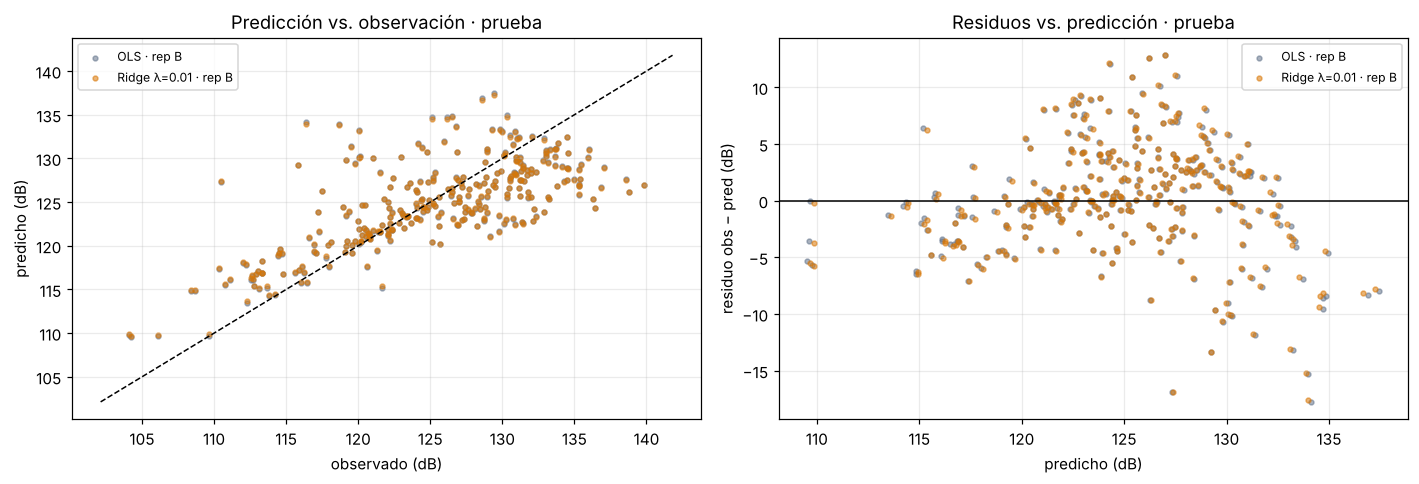
\includegraphics[width=0.85\linewidth]{p6_final.png}
\caption{Airfoil, prueba: predicción frente a observación y residuos frente a predicción (OLS-B y Ridge-B casi se superponen).}\label{fig:p6}
\end{figure}

\textbf{(d) Escenario de generalización.}
Una partición aleatoria de filas mide interpolación dentro del mismo experimento, porque casi toda fila de prueba tiene en desarrollo otras frecuencias del mismo ensayo (misma cuerda, ángulo y velocidad). Para evaluar condiciones nuevas agruparía por ensayo con \texttt{GroupKFold}, o reservaría para prueba valores completos que el modelo nunca vio, como una velocidad o una cuerda. No hice esa evaluación, así que no puedo afirmar que el modelo generalice a esas condiciones.

En Airfoil regularizar no ayuda: los candidatos empatan en CV y en prueba, y Lasso no anula ningún coeficiente. Ridge quedó elegido por la regla de desempate y OLS sería igual de defendible; la mejora que sí se observa viene de la representación. Los coeficientes deben leerse como asociaciones dentro de este diseño experimental y no como efectos causales.

% ---------------------------------------------------------------------
\subsection*{Problema 7. Clasificación temporal y política de alertas}
El objetivo es avisar con dos horas de anticipación qué vuelos se van a retrasar. Los retrasos son pocos (2--4\%), y eso obliga a cuidar tres cosas: no usar información del futuro, medir con métricas adecuadas para clases desbalanceadas y escoger el umbral de alerta según los costos y la capacidad de atender alertas.

\textbf{(a) Datos, diccionario y partición.}
Uso \texttt{generar\_vuelos(n=9600, seed=2026)} sin cambios y $Y=\mathbb 1\{\texttt{min\_retraso}\ge15\}$. Todo el protocolo (partición temporal, \emph{pipeline}, fuga, métricas, umbrales y evaluación final) sigue el taller de vuelos de clase~\cite{nbvuelos}. Dos horas antes del vuelo se conocen la hora programada, la distancia, la lluvia y el viento pronosticados, la ocupación y el tráfico programados, la aerolínea y el origen. \texttt{min\_retraso} solo se conoce después y se usa únicamente como etiqueta; \texttt{fecha\_prediccion} sirve solo para ordenar y partir.

Ordeno por fecha, corto al 60\% y al 80\% y descarto las 24 filas anteriores a cada corte. Quedan entrenamiento V00000--V05735 (5736 filas, del 2024-01-01 al 2024-08-26), validación V05760--V07655 (1896) y prueba V07680--V09599 (1920), y un \texttt{assert} comprueba que hay 25\,h entre conjuntos consecutivos. En entrenamiento hay 140 retrasos (2.44\%) y cerca de 6\% de faltantes en lluvia, viento, ocupación y aerolínea; el tráfico y la prevalencia crecen con el tiempo. El preprocesamiento (mediana y estandarización para las numéricas; moda y one-hot con \texttt{handle\_unknown='ignore'} para las categóricas~\cite[secc.~1.5.3 y 1.5.5]{pml1}) se ajusta siempre dentro del entrenamiento correspondiente.

\textbf{(b) Comparación por validación cruzada temporal.}
Comparo mi logística L2 sin ponderar (\texttt{LogisticRegressionGD}) con la ponderada de scikit-learn, \texttt{LogisticRegression(class\_weight='balanced')}, como en el notebook de clase. Sus pesos son $a_c=N/(2N_c)$, calculados en cada entrenamiento, y cumplen $\sum_na_{y_n}=N$. scikit-learn minimiza $C\sum_na_{y_n}\ell_n+\frac12\lVert w\rVert^2$ sin penalizar el intercepto; dividiendo por $CN$ se obtiene $\frac1N\sum_na_{y_n}\ell_n+\frac{\lambda_2}{2}\lVert w\rVert^2$ con $C=1/(N\lambda_2)$, la misma traducción de la Tabla~\ref{tab:equiv}.

Los pliegues salen de \texttt{TimeSeriesSplit(4, gap=24)}: el conjunto de ajuste crece y siempre precede al de evaluación, y los cuatro pliegues evaluados contienen ambas clases (entre 27 y 31 positivos). El criterio de selección es la AP (área bajo precisión--recall), que se concentra en los positivos y funciona bien con clases desbalanceadas.

\begin{table}[h]\centering\small
\caption{AP media (desviación) en CV temporal. Referencia constante: AP 0.026. No alertar: costo 0.31 por vuelo.}
\begin{tabular}{lccccc}\toprule
$\lambda_2$ & $10^{-3}$ & $10^{-2}$ & $10^{-1}$ & 1 & 10\\\midrule
Sin ponderar & 0.229 (0.06) & 0.236 (0.08) & 0.216 (0.08) & 0.209 (0.08) & 0.209 (0.08)\\
Ponderada & 0.226 (0.07) & 0.238 (0.08) & \textbf{0.246 (0.10)} & 0.223 (0.09) & 0.211 (0.08)\\\bottomrule
\end{tabular}\end{table}

Sin empates, gana la logística ponderada con $\lambda_2=0.1$. Su ventaja de 0.011 es pequeña al lado de la dispersión entre pliegues, así que la tomo como resultado de aplicar la regla y no como una superioridad demostrada. La ponderación, además, empeora la log-loss (0.46 frente a 0.10) y el Brier.

\textbf{(c) Contraexperimento de fuga y diagnóstico en validación.}
Con el ganador y los pliegues fijos, comparo ajustar el preprocesamiento una sola vez con todo el entrenamiento antes de la CV (versión contaminada) contra ajustarlo dentro de cada pliegue (versión correcta). La versión contaminada usa, por ejemplo, una mediana de tráfico de 48.21 en lugar de valores entre 46.18 y 47.43. Aun así, la diferencia de AP (contaminada menos correcta) es $-0.002$ en promedio (de $-0.005$ a $+0.0002$) y la de log-loss $-0.0008$. Que la diferencia sea pequeña o negativa no demuestra que no haya fuga: la fuga es un defecto del procedimiento, porque usa información que no existiría al momento de predecir, y en este caso lo que se filtra predice poco y la deriva temporal puede mover el resultado en cualquier sentido. Estos números no intervienen en la selección.

En validación la prevalencia es 3.9\%. El modelo sin ponderar obtiene AP 0.392, ROC-AUC 0.851, log-loss 0.126 y Brier 0.032; el ponderado, AP 0.394, ROC-AUC 0.853, log-loss 0.535 y Brier 0.178. La AP, que suma por escalones, y el área trapezoidal bajo la curva PR, que une los puntos con rectas, difieren en cerca de 0.002.

Para la calibración uso 5 grupos por cuantiles (379--380 casos; 0/2/9/10/53 y 0/2/9/9/54 positivos; sin probabilidades repetidas). El modelo sin ponderar queda cerca de la diagonal salvo en el último grupo (0.090 frente a 0.140). El ponderado sobrestima mucho (0.15--0.70 frente a 0--0.14): al dar a cada retraso un peso unas 40 veces mayor ($a_1/a_0=N_0/N_1$), aprende probabilidades infladas. Ordena bien los vuelos, pero sus salidas no se pueden leer como probabilidades. Mantengo el ganador.

\textbf{(d) Política de alertas.}
Si $p$ fuera la probabilidad verdadera de retraso, alertar costaría en promedio $1\cdot(1-p)$ por la falsa alarma y no alertar costaría $12p$ por el retraso no avisado. Conviene alertar cuando $12p\ge1-p$, es decir, cuando $p\ge1/13\approx0.077$. Esta regla decide vuelo por vuelo y no limita el número de alertas; es la idea de la diapositiva~32 de~\cite{clase5}, según la cual mover $\tau$ cambia la decisión pero no el modelo.

Con las probabilidades de validación del ganador evalúo 1898 umbrales: todos los valores únicos más ``alertar a todos'' ($\tau=0$) y ``no alertar'' ($\tau=+\infty$), marcados con un indicador de modo extremo. Ninguno cumple simultáneamente recall $\ge0.80$ y alertas $\le15\%$, de modo que el resultado es una inviabilidad empírica. Con un máximo de 15\% de alertas el mejor recall es 0.635 ($\tau=0.6351$, 14.0\%), y llegar a recall 0.80 exige alertar al menos al 34.6\% ($\tau=0.4546$). Congelo el umbral de menor costo sin restricciones, $\tau=0.6351112239347184$ (costo 0.286), como referencia diagnóstica y no como política aprobada.

Como comparación, $\tau=0.5$ da recall 0.77 con 28\% de alertas (costo 0.358). El umbral $\tau=1/13$ presupone probabilidades correctas, y con las probabilidades infladas del modelo ponderado alerta al 98.5\% de los vuelos (costo 0.946), peor que no alertar (0.468). Lo que falla ahí es el supuesto de probabilidades bien calibradas, no la regla de Bayes.

\begin{figure}[h]\centering
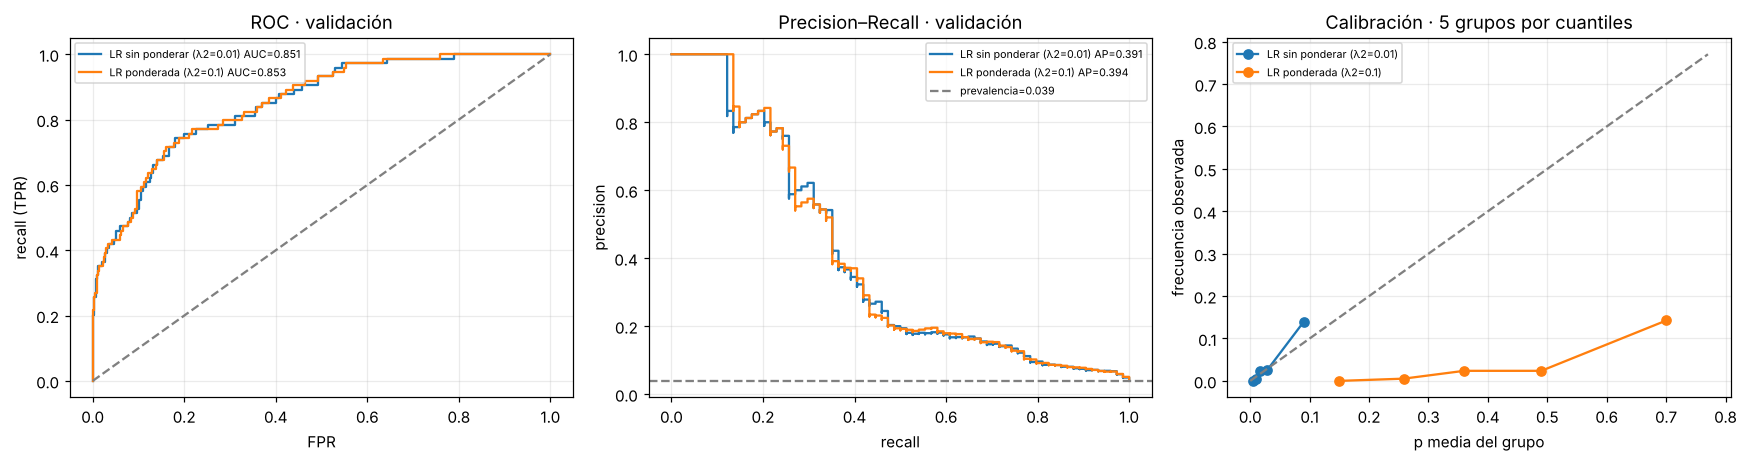
\includegraphics[width=\linewidth]{p7_validacion.png}\\[2pt]
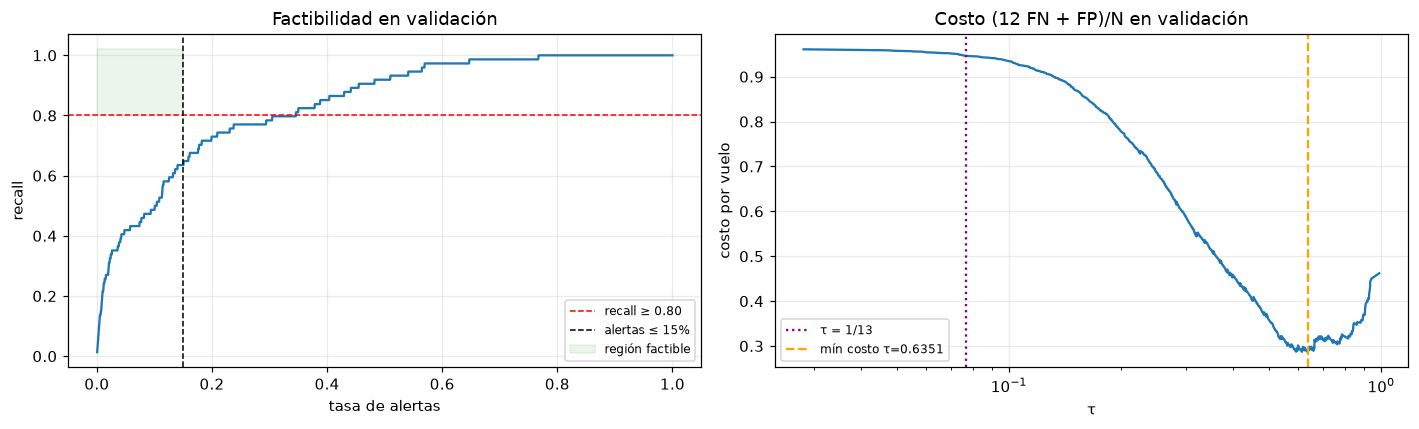
\includegraphics[width=0.78\linewidth]{p7_umbrales.png}
\caption{Vuelos, validación: ROC, PR y calibración (5 grupos por cuantiles) de los dos candidatos; factibilidad recall--alertas y costo por umbral del ganador.}
\end{figure}

\textbf{(e) Evaluación final en prueba.}
Antes de abrir la prueba guardé un manifiesto JSON con variables, preprocesamiento, parámetros, regla y umbral sin redondear, y no reentreno con validación. La prueba tiene 71 retrasos en 1920 vuelos. Las métricas de probabilidad son AP 0.409, ROC-AUC 0.869, log-loss 0.561 y Brier 0.191, iguales para las tres políticas porque no dependen del umbral (lo verifica un \texttt{assert}). Las métricas de decisión las calculo con NumPy a partir de TP, TN, FP y FN, y las contrasto con \texttt{confusion\_matrix} (Tabla~\ref{tab:p7}).

\begin{table}[h]\centering\small
\caption{Evaluación única en prueba (alertas por cada 1000 vuelos).}\label{tab:p7}
\begin{tabular}{lcccccccccc}\toprule
Política & TP & FP & FN & TN & Prec. & Recall & Espec. & F1 & Acc. & Costo / Alertas\\\midrule
$\tau=0.5$ & 57 & 565 & 14 & 1284 & 0.092 & 0.803 & 0.694 & 0.165 & 0.698 & 0.382 / 324\\
$\tau=1/13$ & 71 & 1821 & 0 & 28 & 0.038 & 1.000 & 0.015 & 0.072 & 0.052 & 0.948 / 985\\
$\tau=0.6351$ (diagn.) & 50 & 234 & 21 & 1615 & 0.176 & 0.704 & 0.873 & 0.282 & 0.867 & 0.253 / 148\\\bottomrule
\end{tabular}\end{table}

Tampoco en prueba hay una política que cumpla las dos restricciones. La diagnóstica respeta la capacidad (148 alertas por cada 1000) y tiene el menor costo, pero su recall es 0.70. El umbral se eligió con solo 74 positivos en validación, de modo que cada uno mueve el recall cerca de 1.4 puntos, y además la prevalencia y el tráfico cambian con el tiempo; lo que se cumplía en validación no tenía por qué cumplirse en prueba. No modifico la política después de ver la prueba. Con estas variables la meta conjunta no es alcanzable, y lo razonable sería revisar la capacidad de atención de alertas o conseguir información adicional.

% =====================================================================
\section*{Conclusiones}
\begin{itemize}
\item Igualando los objetivos, mis implementaciones coinciden con scikit-learn a precisión de máquina. Cuando la solución no es única, la verificación debe hacerse sobre el objetivo y las predicciones y no sobre los coeficientes.
\item La regularización intercambia varianza por sesgo. Fue útil con datos mal condicionados (simulación con $\rho=0.9$) y no aportó en Airfoil, que está bien condicionado y donde pesó más la representación.
\item Seleccionar las variables correctas y predecir bien resultaron ser objetivos distintos.
\item Con clases desbalanceadas, ordenar bien (AP, ROC-AUC) no implica tener probabilidades calibradas; el umbral de Bayes solo funciona con probabilidades correctas, y cuando una restricción operativa no se puede cumplir hay que reportarlo así.
\end{itemize}

\textbf{Reproducibilidad.} En la última ejecución (\equipo), desde un kernel limpio, los notebooks 01, 02 y 03 tardan \tiempoUno, \tiempoDos{} y \tiempoTres{} (medido con \texttt{jupyter nbconvert -{}-execute}, incluyendo el arranque del kernel). Las versiones y el orden de ejecución están en el README.


% =====================================================================
\section*{Atribución, contribuciones y uso de IA generativa}
\textbf{Código adaptado de \texttt{Regresion\_lineal\_logistica\_regularizacion.ipynb} (notebook de clase).}
\begin{itemize}
\item \texttt{LinearRegressionScratch} $\to$ \texttt{LinearRegressionGD} y su clase base \texttt{\_Linear}. Conservé el descenso por gradiente sobre MSE/2 y la parada por la norma del gradiente. Cambié: el vector aumentado $\theta=(b,w)$ con la matriz $P$ para agregar L2 sin penalizar $b$; la tasa \texttt{learning\_rate} por $\eta=1/L$ calculado con la norma espectral (por eso \textbf{eliminé el parámetro de tasa manual}, que ya no se usaba); el inicio en $\theta=0$ en vez de $b=\bar y$; y agregué historial del objetivo, motivo de parada, revisión de entradas y guardado en JSON (Problema 4a--4b).
\item \texttt{LogisticRegressionScratch} $\to$ \texttt{LogisticRegressionGD}. Mantuve la estructura scores--probabilidades--error--gradiente y agregué L2, \texttt{predict(X, threshold)} y \texttt{log\_loss} calculada desde el score. Para el modelo ponderado del Problema~7 uso \texttt{LogisticRegression(class\_weight='balanced')} de scikit-learn, como \texttt{construir\_pipeline} del taller de vuelos.
\item \texttt{fit\_regularized} $\to$ función \texttt{gradiente\_proximal} y clase \texttt{LassoRegression}. Tomé el paso de gradiente seguido del umbral suave y la parada por $\lVert\theta^+-\theta\rVert/\eta$. Lo separé en una función que usan los tres modelos iterativos (para no repetir el algoritmo) y apliqué el umbral solo a $w$ con $\eta\lambda_1$; agregué \texttt{proximal\_residual} para verificar la optimalidad de Lasso.
\item \texttt{sigmoid} y \texttt{binary\_cross\_entropy} $\to$ \texttt{sigmoid} (sin cambios) y \texttt{logistic\_loss\_terms}, que devuelve la pérdida de cada observación con la misma fórmula \texttt{np.logaddexp} en lugar de su promedio.
\item \texttt{prepare\_data} y la celda de descarga de Airfoil $\to$ \texttt{ajustar\_predecir} y la celda de carga del Notebook~2. Reutilicé la URL, los nombres de columnas y la idea de ajustar el \texttt{StandardScaler} solo con entrenamiento; agregué el \texttt{id} estable, el manifiesto de la partición y los pliegues de validación cruzada (Problema 6).
\end{itemize}
\textbf{Código adaptado de \texttt{Taller\_clasificacion\_vuelos.ipynb} (notebook de clase).}
\begin{itemize}
\item \texttt{generar\_vuelos}: copia literal, sin cambiar el mecanismo; solo paso \texttt{seed=2026} explícito.
\item \texttt{separar\_por\_tiempo} $\to$ celda de partición del Notebook~3: mismos cortes 60/80\% y gap de 24 filas; agregué \texttt{id\_vuelo}, el manifiesto \texttt{p7\_particiones.csv} y la comprobación de las 25\,h.
\item \texttt{construir\_pipeline} $\to$ \texttt{crear\_prep}, \texttt{crear\_modelo}, \texttt{ajustar} y \texttt{probas}: el mismo \texttt{ColumnTransformer}, separado del clasificador porque el modelo sin ponderar es mi \texttt{LogisticRegressionGD}; el ponderado es el mismo \texttt{LogisticRegression(class\_weight='balanced')} de clase con $C=1/(N\lambda_2)$.
\item \texttt{comparar\_fuga} $\to$ celda del contraexperimento: misma comparación global vs.\ por pliegue, con mi modelo, la log-loss y las estadísticas de tráfico usadas.
\item \texttt{tabla\_umbrales} y \texttt{seleccionar\_umbral} $\to$ \texttt{tabla\_umbrales} y la celda de política: agregué $\tau=0$ y $\tau=+\infty$ con indicador de modo, el costo $(12FN+FP)/N$, la restricción de alertas, los desempates del 7d y el reporte de inviabilidad.
\item \texttt{metricas\_manuales} y \texttt{comparar\_politicas} $\to$ celda de evaluación final: TP/TN/FP/FN con NumPy verificados con \texttt{confusion\_matrix}; quité el recorte de probabilidades en la log-loss y agregué especificidad, Brier, costo y alertas por cada 1000 vuelos.
\end{itemize}
{\sloppy Son míos, sin código base del curso: \texttt{OLSRegression}, \texttt{RidgeRegression}, \texttt{numerical\_gradient}, \texttt{relative\_gradient\_error}, las 30 pruebas del Notebook~1, la simulación del Problema 5 y los bucles de validación cruzada de los Problemas 6 y 7.\par}

\textbf{Contribuciones.} Trabajo individual (Juan José Jiménez Maya): derivaciones, implementación, experimentos e informe.

\textbf{Uso de IA generativa.} Utilicé IA generativa como apoyo para encaminar las demostraciones (redacté el planteamiento original en Obsidian y utilicé Claude exclusivamente para transcribir y formatear el texto de Markdown a LaTeX), y también la utilicé para adaptar lo necesario del código base de los talleres a las necesidades y requerimientos específicos de esta implementación. Ninguna salida de la IA sustituye las demostraciones, las pruebas numéricas o los resultados ejecutados, que se reproducen al ejecutar los notebooks desde un kernel limpio.

\begin{thebibliography}{9}\small\setlength{\itemsep}{1pt}
\bibitem{clase5} Curso de Aprendizaje Automático, UNAL Medellín (2026-2S). \emph{Regresión lineal y regresión logística}, clase teórica de la semana~5 (diapositivas).
\bibitem{nbreg} Curso de Aprendizaje Automático (2026-2S). Notebook \texttt{Regresion\_lineal\_logistica\_regularizacion.ipynb}.
\bibitem{nbeda} Curso de Aprendizaje Automático (2026-2S). Notebook \texttt{Clase\_practica\_EDA\_para\_Machine\_Learning.ipynb}.
\bibitem{nbvuelos} Curso de Aprendizaje Automático (2026-2S). Notebook \texttt{Taller\_clasificacion\_vuelos.ipynb}.
\bibitem{pml1} Murphy, K.\,P. (2022). \emph{Probabilistic Machine Learning: An Introduction}. MIT Press (versión en línea de 2025), caps.~1--4.
\bibitem{airfoil} Brooks, T., Pope, D., Marcolini, M. (1989). \emph{Airfoil Self-Noise}. UCI Machine Learning Repository, doi:10.24432/C5VW2C.
\bibitem{sklearn} Pedregosa, F. et al. (2011). Scikit-learn: Machine learning in Python. \emph{JMLR} 12, 2825--2830.
\end{thebibliography}
\end{document}
